\documentclass[a4paper]{article}
\usepackage[spanish]{babel}
\usepackage[utf8]{inputenc}
\usepackage{charter}   % tipografia
\usepackage{graphicx}
%\usepackage{makeidx}
\usepackage{paralist} %itemize inline

%\usepackage{float}
%\usepackage{amsmath, amsthm, amssymb}
%\usepackage{amsfonts}
%\usepackage{sectsty}
%\usepackage{charter}
%\usepackage{wrapfig}
%\usepackage{listings}
%\lstset{language=C}


\usepackage{color} % para snipets de codigo coloreados
\usepackage{fancybox}  % para el sbox de los snipets de codigo

\definecolor{litegrey}{gray}{0.94}

% \newenvironment{sidebar}{%
% 	\begin{Sbox}\begin{minipage}{.85\textwidth}}%
% 	{\end{minipage}\end{Sbox}%
% 		\begin{center}\setlength{\fboxsep}{6pt}%
% 		\shadowbox{\TheSbox}\end{center}}
% \newenvironment{warning}{%
% 	\begin{Sbox}\begin{minipage}{.85\textwidth}\sffamily\lite\small\RaggedRight}%
% 	{\end{minipage}\end{Sbox}%
% 		\begin{center}\setlength{\fboxsep}{6pt}%
% 		\colorbox{litegrey}{\TheSbox}\end{center}}

\newenvironment{codesnippet}{%
	\begin{Sbox}\begin{minipage}{\textwidth}\sffamily\small}%
	{\end{minipage}\end{Sbox}%
		\begin{center}%
		\vspace{-0.4cm}\colorbox{litegrey}{\TheSbox}\end{center}\vspace{0.3cm}}



\usepackage{fancyhdr}
\pagestyle{fancy}

%\renewcommand{\chaptermark}[1]{\markboth{#1}{}}
\renewcommand{\sectionmark}[1]{\markright{\thesection\ - #1}}

\fancyhf{}

\fancyhead[LO]{Sección \rightmark} % \thesection\ 
\fancyfoot[LO]{\small{Nombre Apellido, Nombre Apellido, Nombre Apellido}}
\fancyfoot[RO]{\thepage}
\renewcommand{\headrulewidth}{0.5pt}
\renewcommand{\footrulewidth}{0.5pt}
\setlength{\hoffset}{-0.8in}
\setlength{\textwidth}{16cm}
%\setlength{\hoffset}{-1.1cm}
%\setlength{\textwidth}{16cm}
\setlength{\headsep}{0.5cm}
\setlength{\textheight}{25cm}
\setlength{\voffset}{-0.7in}
\setlength{\headwidth}{\textwidth}
\setlength{\headheight}{13.1pt}

\renewcommand{\baselinestretch}{1.1}  % line spacing


% \setcounter{secnumdepth}{2}
\usepackage{underscore}
\usepackage{caratula}
\usepackage{url}


% ******************************************************** %
%              TEMPLATE DE INFORME ORGA2 v0.1              %
% ******************************************************** %
% ******************************************************** %
%                                                          %
% ALGUNOS PAQUETES REQUERIDOS (EN UBUNTU):                 %
% ========================================
%                                                          %
% texlive-latex-base                                       %
% texlive-latex-recommended                                %
% texlive-fonts-recommended                                %
% texlive-latex-extra?                                     %
% texlive-lang-spanish (en ubuntu 13.10)                   %
% ******************************************************** %



\begin{document}


\thispagestyle{empty}
\materia{Organización del Computador II}
\submateria{Segundo Cuatrimestre de 2014}
\titulo{Trabajo Práctico II}
\subtitulo{subtitulo del trabajo}
\integrante{Alejandro Mignanelli}{609/11}{minga_titere@hotmail.com}
\integrante{Franco Negri}{893/13}{franconegri2004@hotmail.com}
\integrante{Federico Suárez}{610/11}{elgeniofederico@gmail.com}

\maketitle
\newpage

\thispagestyle{empty}
\vfill
\begin{abstract}
En el presente trabajo se describe la problemática de procesar información de manera eficiente cuando los mismos requieren:
\begin{enumerate}
\item Transferir grandes volumenes de datos.
\item Realizar las mismas instrucciones sobre un set de datos importante.
\end{enumerate}

\end{abstract}

\thispagestyle{empty}
\vspace{3cm}
\tableofcontents
\newpage

%\normalsize
\newpage

\section{Objetivos generales}

El objetivo de este Trabajo Práctico es mostrar las variaciones en la performance que suceden al utilizar instrucciones SIMD en comparación con código C con diversos grados de optimización realizados por el compilador cuando se manejan grandes volúmenes de datos que requieren un procesamiento similar.

Para ello se realizarán distintos experimentos sobre cuatro filtros de fotos, Cropflip, Bandas, Sierpinski y Motion Blur, tanto en código assembler, que aproveche las instrucciones SSE brindadas para los procesadores de arquitectura Intel, como en código C, al que se le aplicarán los distintos flags de optimización -O0 (predeterminado), -O1, -O2 y -O3.

El primer filtro, Cropflip, se utilizará para mostrar cuanto mejora la performance al utilizar los registros XMM para transferir grandes cantidades de información.

El segundo, tercer y cuarto filtro, se centrarán en la variación de performance (en comparación al código en C) al utilizar instrucciones SIMD, no sólo para transferir grandes volúmenes de datos sino también para procesarlos en forma paralela, es decir, realizar diversos cálculos (sumas, multiplicaciones, divisiones) tanto en representación de enteros como punto flotante.

\section{Preambulo}

\subsection{Calidad de las Mediciones}
Para este experimento vamos a ver cómo se pueden ver afectados nuestros algoritmos frente a diversos factores de ruido e interferencias que podrían alterar nuestras mediciones.

Para este experimento se utilizó un procesador Intel Atom, de 2 núcleos a 1.6 GHZ con Hyper-Threading, por lo que la cantidad de núcleos lógicos asciende a 4. Por otro lado, para que las pruebas sean mas concisas y exactas, se deshabilitó el scaling dinamico del CPU, ya que esto podría generar ruido innecesario en nuestras mediciones.

Procedimos a tomar 10 mediciones para cada una de las versiones del cropflip, tanto con 4 loops corriendo en paralelo como sin los mismos. La medida de tiempo será a partir de este momento y para siempre la cantidad de ciclos de clock del procesador. Lo que se obtiene es el siguiente gráfico:
\\
\begin{figure}[h!]
  \begin{center}
  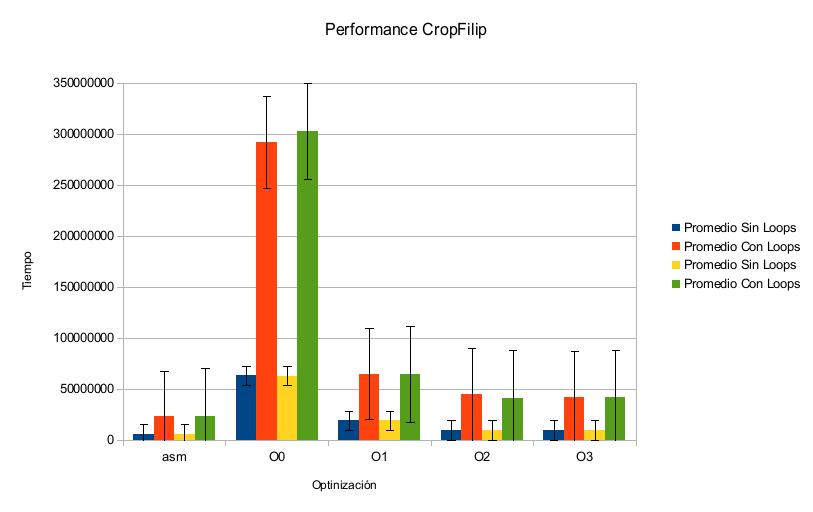
\includegraphics[scale=0.66]{Graficos1.4/1.3/per.jpg}
  \label{nombreparareferenciar1}
  \end{center}
\end{figure}
\\

Lo que se observa aquí es que al correr las pruebas con loops en segundo plano, la performance se ve afectada de forma negativa aumentando el tiempo de ejecución. Además podemos ver que los outliers cuando hay ruido tienen un mayor impacto en el rendimiento mientras que cuando no hay loops de fondo, su impacto es apenas notable. También se puede apreciar que la optimización -O1 es la que más se ve perjudicada por el ruido de los loops. Con respecto a la varianza, se puede percibir fácilmente que el ruido la dispara considerablemente, es decir, aumenta abismalmente la dispersión de los datos. Por otro lado, se ve que los outliers tuvieron una mayor repercusión en la varianza de los casos sin loops.

\newpage

\section{Experimentación}

\subsection{Desensamblado de código C y Optimización}

Comenzamos analizando el código de Cropflip realizado en C.

Este básicamente solo mueve datos de un lugar de la RAM a otros, sin afectar mayormente la imagen.

Realizamos un objdump para ver el código que genera el compilador gcc. Al desensamblar el código pudimos observar, primero que nada, que C guarda todos los parámetros en la pila y además está escribiendo en memoria todas las variables locales utilizadas, lo cual es innecesario ya que pueden ser almacenadas en registros.

También puede observarse que C utiliza saltos incondicionales, lo que puede sugerir que intenta sacar provecho al sistema de predicción de saltos.

Ademas C genera, luego de la función, un montón de secciones que comienzan con debug_xxx. Estas secciones sirven para ser interpretadas por GDB u otros debuggers.

Como ya dijimos, el código podría optimizarse para no realizar tantos accesos a memoria innecesarios guardando variables locales por ejemplo en registros, lo cual disminuiría el tiempo de ejecución.

Luego de esto, procedemos a compilar el código utilizando el flag -O1, y nuevamente realizamos un objdump para ver el código desensamblado. Se observa que ahora el mismo solo realiza los accesos a memoria mínimos indispensables, utilizando los registros para guardar los datos. Además el código es más compacto, y resulta mas claro de leer. Además precalcula los valores que serán utilizados muchas veces, lo que aumenta la performance, principalmente en casos de instancias grandes.

Los otros flags de optimización son -O2, -O3, -Og, -Os, -Ofast. También podemos encontrar los flags -msse, -msse2, -msse3, -mmmx, -m3dnow, pero al intentar compilar con varios de ellos vimos que gcc no utilizó instrucciones SIMD.

Tres nombres de optimizaciones son: -fipa-profile, -fipa-reference ,-fmerge-constants .

\newpage

\section{Cropflip}

\subsection{Diferencias de performance en Cropflip}
En el siguiente experimento se medirán las performances tanto de nuestro algoritmo en assembler, implementado para sacar provecho de las instrucciones SSE de Intel, como una versión alternativa hecha en C con diversos grados de optimización a cargo del compilador.

El algoritmo de Cropflip en assembler es muy sencillo. Simplemente movemos 128-bits de la imagen a un xmm y de allí al destino, que previamente ha sido seteado para colocar los bits en el lugar correcto. De esta manera, podremos mover de una sola vez, 16 bytes, lo que corresponde a 4 píxels de la imagen.

Dado que la cantidad de columnas es siempre múltiplo de 4, o sea, siempre tenemos 4 bytes para tomar, no es necesario chequear otros casos borde.

Las pruebas de performance, realizadas de la misma manera en que concluímos la anterior sección, se realizaron corriendo 4 loops en paralelo junto con los algoritmos de manera de minimizar el ruido y luego quitando los outliers.

Lo obtenido en los tests puede verse en el siguiente gráfico:

\begin{figure}[h!]
  \begin{center}
	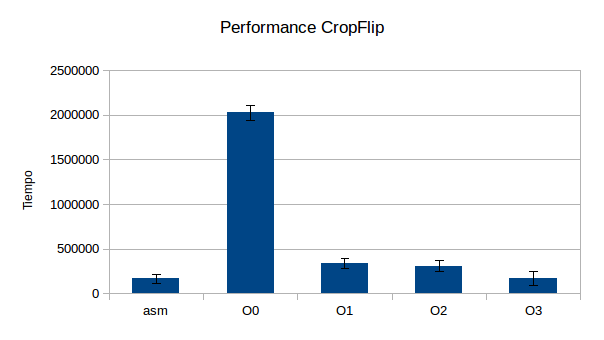
\includegraphics[scale=0.66]{Graficos1.4/crop/per.jpg}
	\label{nombreparareferenciar5}
  \end{center}
\end{figure}

En este caso la performance de nuestro algoritmo es ligeramente menor al código de mayor grado de optimización de C. Creemos que esto se debe a que al ser un código muy simple, el cual sólo mueve datos de un lugar a otro, el tiempo de ejecución de ambos es muy similar y la diferencia se la atribuimos al ruido. La varianza de mayor nivel es la optimización O0, mientras que las demás tienen un nivel relativamente bajo de dispersión. Observamos que sin embargo, la nuestra es la mayor de las restantes, lo que favorece nuestra proposición sobre el ruido.

\newpage

\subsection{cpu vs. bus de memoria en Cropflip}

Para este experimento lo que hicimos fue agregar instrucciones aritméticas y ver como esto influía en el tiempo de ejecución.

También hicimos lo mismo pero con instucciones de lectura-escritura en memoria. 

Probamos agregando $4$, $8$ y $16$ instrucciones de cada una por separado y comparamos las performance entre sí y con la versión original.

Lo que obtuvimos fue lo siguiente:

\begin{figure}[h!]
  \begin{center}
  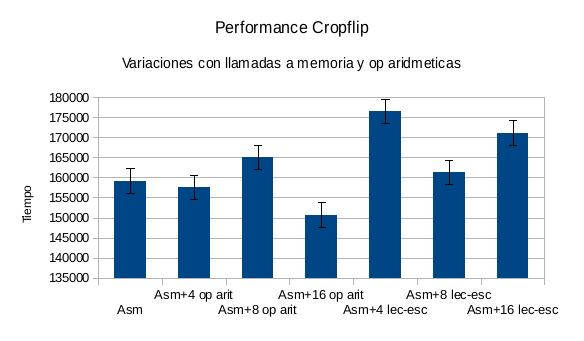
\includegraphics[scale=0.66]{Graficos1.5/crop/per.jpg}
  \label{nombreparareferenciar1}
  \end{center}
\end{figure}

==conculsión!!!==

\newpage
\section{Sierpinski}

\subsection{Idea general del algoritmo}

Ahora analizamos el algoritmo del Sierpinski. En este caso, el algoritmo ya es un poco más complejo. Necesitamos calcular para cada píxel un coeficiente diferente, que dependerá de la posición (i,j) de cada píxel.
\\
Luego para poder paralelizar de alguna manera el algoritmo en C y sacar provecho a los registros xmm, es necesario calcular 4 coeficientes a la vez y multiplicárselos a sus respectivos píxels.
\\
Luego la idea del algoritmo será algo así:

\begin{itemize}
\item En la sección data guardamos una constante con el valor 255 brodcasteado en punto flotante.
\item Previo al ciclo, guardamos este valor en un registro.
\item Ya dentro del ciclo, leemos 4 píxels y los guardamos en un xmm.
\item A continuación calculamos de manera paralela para cada píxel el coeficiente correspondiente.
\item Primero, realizamos la división de i por la cantidad de filas y j por la cantidad de columnas, para la cual previamente pasamos de entero a punto flotante.
\item Multiplicamos ambos valores por 255 y luego convertimos a entero con truncamiento.
\item Realizamos un xor entre ambos y despues, volvemos a convertir a punto flotante para dividir por 255.
\item Ya con los coeficientes calculados, solo nos resta multiplicar cada uno por el píxel correspondiente.
\item Para ello desempaquetamos cada byte de cada píxel leido a word, y luego de word a dword, para así convertirlo a punto flotante.
\item Una vez hecha la conversión, brodcasteamos cada coeficiente para poder multiplicarlo por el píxel correspondiente.
\item Luego convertimos a entero nuevamente y empaquetamos todo de dword a word y de word a byte.
\item Y finalmente movemos los píxels procesados al destino.
\end{itemize}

\subsection{Diferencias de performance en Sierpinski}

Los resultados comparativos de performance para este algoritmo comparado con uno desarrollado en C fueron los siguientes:

\begin{figure}[h!]
  \begin{center}
  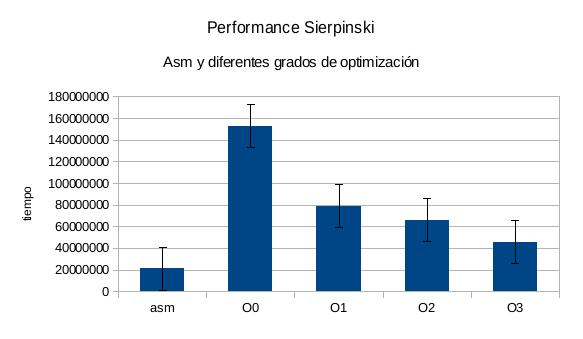
\includegraphics[scale=0.66]{Graficos1.4/sie/per.jpg}
  \label{nombreparareferenciar7}
  \end{center}
\end{figure}

\newpage

Puede verse que en este caso nuestro modelo que toma y calcula de a 4 píxels utilizando instrucciones SIMD es incluso mejor que la versión de C con mayor grado de optimización. Y las varianzas son similares a excepción de la optimización O0 que es un poco mayor.

\newpage
\subsection{CPU vs. Bus de memoria en Sierpinski}

Realizamos el mismo experimento que hicimos para cropflip, es decir, agregando instrucciones aritmeticas y de lectura escritura y comparando las performances.

Graficando lo obtenido:

\begin{figure}[h!]
  \begin{center}
  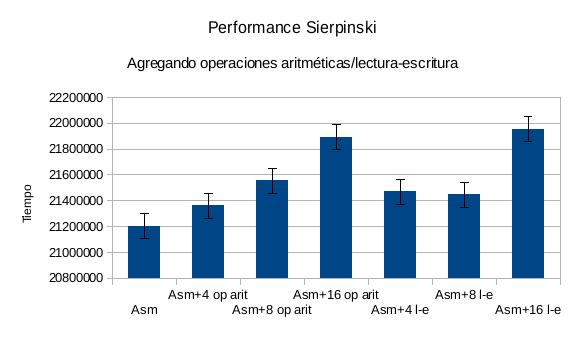
\includegraphics[scale=0.66]{Graficos1.5/sie/per.jpg}
  \label{nombreparareferenciar1}
  \end{center}
\end{figure}

Se puede ver que Sierpinski disminuye su performance de una manera similar cuando se le agregan más operaciones aritméticas o de lectura/escritura de memoria. Viendo la varianza, se observa que las instrucciones aritméticas generan un leve aumento de la misma mientras que las operaciones de lectura/escritura producen una mayor dispersión de los datos.
\newpage
\section{Bandas}
\subsection{Idea general del algoritmo}
Para el algoritmo de bandas se nos presenta otro desafío: debemos tomar los tres colores de la imagen(r,g,b), sumarlos, y luego comparar cada uno de ellos para ver si se encuentra en un rango determinado.
\\
Para resolver la primera problemática usaremos las instrucciones $phaddw$, que nos permitirá a través de una suma horizontal, sumar los valores r,g,b de manera cómoda solamente utilizando dos registros.
\\
El segundo problema será comparar estos valores obtenidos en la suma de una manera eficiente. Querríamos compararlos todos a la vez y a partir de esas comparaciones determinar que valores deberá ir en cada píxel. Esta se resolverá utilizando broadcasting. El algoritmo irá comparando en cada paso contra un valor y en caso de cumplirse una condición, restará donde corresponda.


\begin{itemize}
\item  En la sección data tenemos mascaras y constantes brodcasteadas que utilizaremos para hacer las comparaciones.
\item  Ademas en esta sección tenemos una doble qword la cual usaremos para el shuffle final.
\item  Previo al ciclo donde procesamos los píxels, movemos estos datos a registros xmm.
\item  Ya una vez dentro del ciclo, leemos 4 píxels y los guardamos en un xmm.
\item  Desempaquetamos los bytes a word para poder hacer la suma de las componentes de cada píxel sin irnos de la representación.
\item  Hacemos dos sumas horizontales para obtener los cuatro valores  de b.
\item  Luego utilizamos las mascaras para comparar en paralelo cada píxel con el b correspondiente y asignando el valor de rgb segun corresponda.
\item  Nos queda en cada word de la parte baja de un xmm, los 4 valores que se asignaran a cada rgb de cada píxel.
\item  Finalmente, empaquetamos estos valores para volver a byte y los shuffleamos para dejarlos en los lugares correspondiente y lo asignamos en el destino.
\end{itemize}

\subsection{Diferencias de performance en Bandas}

Los resultados de los tiempos comparativos son los siguientes:

\begin{figure}[h!]
  \begin{center}
  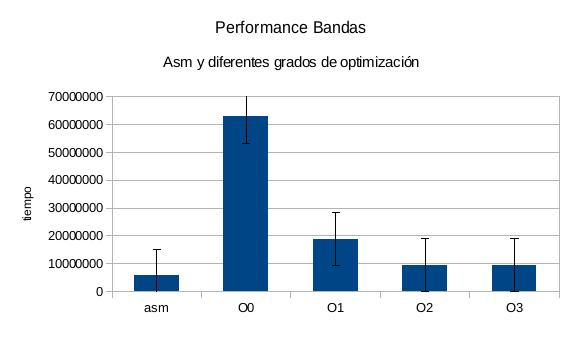
\includegraphics[scale=0.66]{Graficos1.4/ban/per.jpg}
  \label{nombreparareferenciar9}
  \end{center}
\end{figure}

Nuestro algoritmo obtiene una performance mucho mayor a la del código sin optimizar, y una performance un poco mejor al del código C con el mayor grado de optimización. Y con respecto a la varianza, todos tienen una dispersión de datos relativamente baja salvo la optimización O0 cuyo nivel es muy alto.

\newpage
\subsection{Saltos condicionales}

En este experimento veremos como afectan los saltos condicionales a la performance del codigo C compilado con -O1. Para ello lo que haremos es quitar los IFs del codigo dejando solo una banda, luego medir la performance y compararla con la version con saltos.

\begin{figure}[h!]
  \begin{center}
  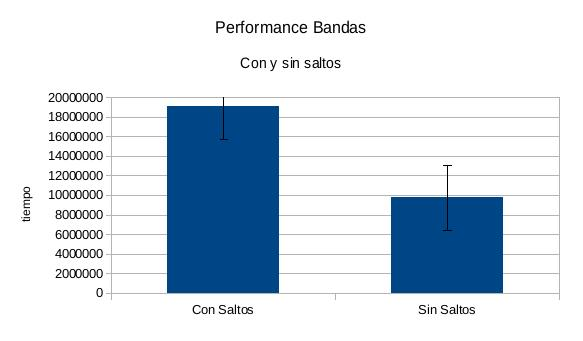
\includegraphics[scale=0.66]{Graficos3.1/per.jpg}
  \label{nombreparareferenciar1}
  \end{center}
\end{figure}

Como se puede ver en el gráfico del promedio, la versión de una sola banda tardó mucho menos con respecto a la versión original. Creemos que esta disminución en el tiempo de ejecución tiene que ver con la predicción de saltos del procesador. Esto se debe a que cuando hay un salto condicional, en principio el procesador no sabe a qué posición de memoria deberá dirigirse. Al haber removido estos saltos, tiene sentido que la performance se haya visto impactada de manera positiva. Con respecto a la varianza se ve que en la versión sin saltos es mucho menor respecto al original, es decir, los valores de la muestra se encuentran relativamente más cercanos al promedio.

\newpage
\subsection{Motion Blur}
\subsection{Idea general del algoritmo}
Para este algoritmo por cada píxel se deben tomar 5 píxels, multiplicar cada uno de los colores por $0.2$ y luego sumarlos.
\\
Para ello debemos tener cuidado de tomar correctamente los casos borde y no aplicar motion blur donde no corresponde.
\\
Una idea general de cómo funciona el algoritmo en assembler es la siguiente:

\begin{itemize}
\item  Tenemos, en la sección datos, el valor $0.2$ brodcasteado que utilizaremos para realizar la multiplicación.
\item  Previo al procesamiento de datos, guardamos en un xmm este valor.
\item  Dentro del ciclo, para procesar el píxel (i,j) tomamos los 4 píxels de las filas $i-2$, $i-1$, $i$, $i+1$ e $i+2$ a partir de la columna $j-2$, $j-1$, $j$, $j+1$ y $j+2$, respectivamente, y almacenamos todo en registros.
\item  Desempaquetamos todo a word para poder hacer la suma sin desbordar.
\item  Luego de realizar las sumas, desempaquetamos a dwords para así poder convertir a punto flotante.
\item  Con la conversión ya hecha, podemos multiplicar cada valor por $0.2$.
\item  Convertimos a entero nuevamente y empaquetamos de dword a word y de word a byte.
\item  Finalmente, copiamos los 4 píxels resultantes al destino. 
\item  Cada vez que termino de recorrer una fila, pongo en negro los siguientes 4 píxels, y las dos primeras y últimas filas las pongo en negro aparte, fuera del ciclo.
\end{itemize}

\subsection{Diferencias de performance en Motion Blur}

Al realizar el testing se obtuvieron los siguientes resultados:

\begin{figure}[h!]
  \begin{center}
  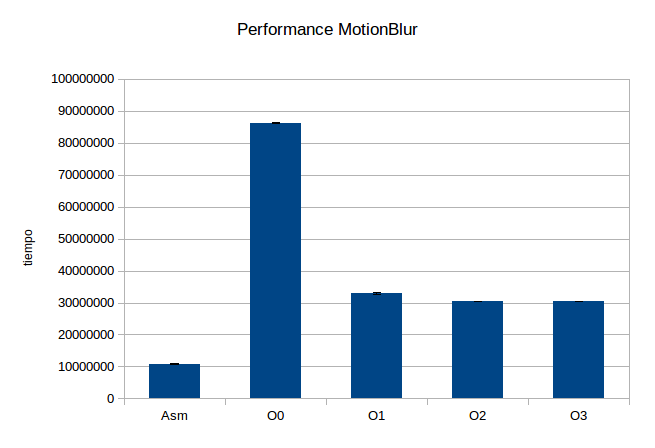
\includegraphics[scale=0.66]{Graficos1.4/mbl/per.jpg}
  \label{nombreparareferenciar11}
  \end{center}
\end{figure}

En este caso nuestro algoritmo supera ampliamente incluso al código C con mayor grado de optimización. De la varianza se ve que nuestro algoritmo tiene una dispersión de datos parecida a la de la optimización O3, mientrás que la optimización O1 es la que más dispersa los datos.

\newpage
\section{Conclusiones y trabajo futuro}

SIMD es una herramienta muy útil para mejorar la performance a la hora de manejar grandes cantidades de datos que requieren un mismo procesamiento, como imágenes o videos, y esto se vio reflejado ampliamente en los resultados de los experimentos realizados en este trabajo. Sin embargo si lo único que necesitamos realizar es un mero movimiento de datos, las diferencias se vuelven imperceptibles con respecto al grado de mayor optimización de C. Sin embargo, un gran poder conlleva una gran responsabilidad y un error de empaquetado o desempaquetado puede resultar en muchas horas de debugging, como por ejemplo desempaquetar dos veces la parte alta de un registro, en vez de desempaquetar la parte baja también.



\end{document}

